\documentclass{article}
\usepackage{amsmath,enumitem,fullpage,graphicx,listings,float,sidecap,setspace,xcolor,wrapfig,booktabs,multirow,subcaption,array,minted,svg,hyperref,xepersian,bidi}

\newcolumntype{C}[1]{>{\centering\arraybackslash}m{#1}}
\definecolor{lg}{HTML}{F4F3F3}
\setlength{\fboxsep}{10pt}
\usemintedstyle{borland}
\hypersetup{
   colorlinks=true,
   linkcolor=blue, % color of internal links
   citecolor=green, % color of links to bibliography
   filecolor=magenta, % color of file links
  urlcolor=cyan % color of external links
}
\setlatintextfont{Vazirmatn}
\settextfont{Vazirmatn}
\begin{document}

\begin{titlepage}
  \centering
  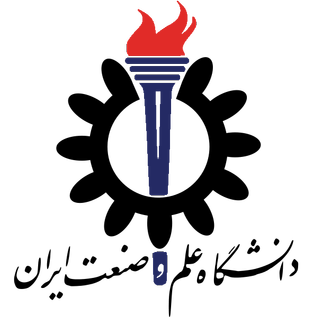
\includegraphics[width=0.5\textwidth]{iust}\par\vspace{1cm}
  {\scshape\LARGE دانشکده مهندسی کامپیوتر \par}
  \vspace{1cm}
  {\huge\bfseries تمرین سری پنچم \par}
  \vspace{1cm}
  {\Large درس مبانی پردازش زبان و گفتار \par}
  \vspace{1cm}
  {\large سینا علی‌نژاد \par}
  \vspace{5cm}
  {\large نیم سال دوم \par}
  {\large سال تحصیلی ۱۴۰۲-۱۴۰۳ \par}
\end{titlepage}
\newpage
\doublespacing
\section*{سوال 1}
سیستم های QA open-domain برای پاسخگویی به سؤالات در مورد طیف گسترده ای از موضوعات طراحی شده اند، بدون اینکه دامنه یا حوزه موضوعی خاصی مشخص شود. این سیستم ها معمولاً بر مقادیر زیادی از داده های بدون ساختار مانند صفحات وب یا کتاب ها متکی هستند و از تکنیک های پردازش زبان طبیعی برای شناسایی اطلاعات مرتبط و ارائه پاسخ استفاده می کنند. پاسخگویی به سؤالات دامنه باز یک کار چالش برانگیز است زیرا سیستم باید قادر به رسیدگی به طیف وسیعی از سؤالات باشد که برخی از آنها ممکن است مبهم یا نامشخص باشند.

از سوی دیگر، سیستم‌های QA closed-domain برای پاسخ‌گویی به سؤالات در یک دامنه یا حوزه موضوعی خاص طراحی شده‌اند. این سیستم‌ها معمولاً با استفاده از منابع داده ساختاریافته، مانند پایگاه‌های داده یا graph knowledge ساخته می‌شوند و برای ارائه پاسخ‌های دقیق به سؤالات مربوط به آن حوزه، بهینه‌سازی شده‌اند. معمولاً پاسخگویی به سؤالات دامنه بسته آسان‌تر از پاسخ‌گویی به سؤالات دامنه باز در نظر گرفته می‌شود، زیرا دامنه سؤالات محدودتر است و منابع داده ساختارمندتر هستند.

\section*{سوال 2}
Machine Reading Comprehension نوعی سیستم هوش مصنوعی است که برای خواندن و درک متن زبان طبیعی طراحی شده است. هدف یک Machine Reading Comprehension استخراج معنا از متن به روشی شبیه به آنچه انسان ها انجام می دهند، با شناسایی مفاهیم کلیدی و روابط بین آنهاست. این سیستمها معمولاً از ترکیبی از تکنیک‌های پردازش زبان طبیعی، مانند Graph Dependency ، Recognition Entity Named ، Tagging Speech of Part و همچنین الگوریتم‌های یادگیری ماشینی برای تحلیل و تفسیر متن استفاده می‌کنند.

ارتباط بین این سیستم و Question-Answering این است که سیستم‌های پاسخ‌گوی سوال اغلب برای شناسایی و استخراج اطلاعات مربوطه از یک مجموعه متن به سیستمهایی برای درک مطلب متکی هستند. به عنوان مثال، در یک سیستم پاسخگویی به سؤالات دامنه باز، سیستم ممکن است از یک دستگاه خواندن درک مطلب برای تجزیه و تحلیل مجموعه بزرگی از صفحات وب یا کتاب ها و شناسایی قسمت هایی که به احتمال زیاد حاوی پاسخ به یک سؤال هستند استفاده کند. سپس سیستم پاسخگویی به سؤال از این اطلاعات برای ایجاد پاسخ به سؤال کاربر استفاده می کند.

به طور مشابه، در یک سیستم پاسخگویی به سؤالات دامنه بسته، سیستم ممکن است از یک سیستم درک مطلب برای تجزیه و تحلیل یک پایگاه داده ساختاریافته یا نمودار دانش و شناسایی نهادها و روابط مرتبط با سؤال کاربر استفاده کند. سپس سیستم پاسخگویی به سؤال از این اطلاعات برای ایجاد پاسخ به سؤال کاربر استفاده می کند.

به طور خلاصه، Machines Reading Comprehension جزء مهم بسیاری از سیستم‌های پاسخ‌گوی پرسش هستند، زیرا سیستم را قادر می‌سازند تا معنی را از متن زبان طبیعی استخراج کند و اطلاعاتی را که بیشترین ارتباط را با سؤال کاربر دارد شناسایی کند.

\section*{سوال 3}
سوالات Factoid سوالاتی هستند که به دنبال یک واقعیت خاص یا بخشی از اطلاعات به عنوان پاسخ هستند. این سؤالات معمولاً یک پاسخ عینی دارند که می تواند از یک مجموعه متن یا پایگاه داده استخراج شود. به عنوان مثال، "پایتخت فرانسه چیست؟" یک سوال Factoid است، زیرا به دنبال یک اطلاعات خاص (پایتخت فرانسه) است که می تواند از یک منبع دانش استخراج شود.

از سوی دیگر، سؤالات Non-Factoid ، سؤالاتی هستند که به دنبال یک واقعیت یا اطلاعات خاصی به عنوان پاسخ نیستند. در عوض، این سوالات ممکن است به دنبال توضیح، نظر یا تفسیر ذهنی از برخی اطلاعات باشند. سوالات Non-Factoid همچنین ممکن است به دنبال فهرستی از موارد یا مقایسه بین موارد مختلف باشند. به عنوان مثال، "مزایا و معایب استفاده از انرژی خورشیدی چیست؟" یک سوال Non-Factoid است، زیرا به دنبال تفسیر ذهنی از مزایا و معایب انرژی خورشیدی است.

تمایز بین سوالات Factoid و Non-Factoid در QA مهم است زیرا انواع مختلف سوالات ممکن است به رویکردهای متفاوتی برای پاسخگویی نیاز داشته باشند. به سؤالات Factoid ممکن است با استفاده از تکنیک هایی مانند Recognition Entity Named ، Extraction Information ، Traversal Graph Knowledge داده شود، در حالی که سؤالات Non-Factoid ممکن است به تکنیک های پردازش زبان طبیعی پیچیده تری مانند Analysis Sentiment ، Summarization Text یا الگوریتمهای یادگیری ماشین نیاز داشته باشند.

\section*{سوال 4}
مزایای ترانسفورماتور:

موازی سازی: ترانسفورماتورها می توانند توالی های ورودی را به صورت موازی پردازش کنند، که باعث می شود آنها سریعتر و کارآمدتر از RNN برای دنباله های طولانی باشند. 

مکانیسم توجه: ترانسفورماتورها از مکانیزم توجهی استفاده می کنند که به آنها اجازه می دهد هنگام تولید یک خروجی به طور انتخابی بر روی قسمت های مختلف توالی ورودی تمرکز کنند. این می تواند دقت و انسجام خروجی را بهبود بخشد. 

وابستگی های دوربرد: ترانسفورماتورها در گرفتن وابستگی های دوربرد در توالی ورودی بهتر از RNN ها هستند، که می تواند برای کارهایی مانند مدل سازی زبان و ترجمه ماشینی مهم باشد.  

انعطاف‌پذیری: ترانسفورماتورها را می‌توان برای طیف وسیعی از وظایف پردازش زبان طبیعی، از جمله مدل‌سازی زبان، ترجمه ماشینی و پاسخ‌گویی به سؤالات استفاده کرد.   


معایب ترانسفورماتورها: 

پیچیدگی: ترانسفورماتورها پیچیده تر از RNN ها هستند، که می تواند پیاده سازی و اشکال زدایی آنها را دشوارتر کند. 

استفاده از حافظه: ترانسفورماتورها می توانند به حافظه بیشتری نسبت به RNN نیاز داشته باشند، که می تواند برای کارهای پردازش زبان طبیعی در مقیاس بزرگ مشکل ایجاد کند. 

زمان آموزش: آموزش ترانسفورماتورها نسبت به RNN ها بیشتر طول می کشد، به خصوص برای کارهای در مقیاس بزرگ. 

عدم تفسیرپذیری: تفسیر مکانیسم توجه در ترانسفورماتورها ممکن است دشوار باشد، که می تواند درک چگونگی پیش بینی مدل را دشوارتر کند.

\section*{سوال 5}
رمزگذاری موقعیتی تکنیکی است که در مدل های مبتنی بر ترانسفورماتور برای ارائه اطلاعات در مورد موقعیت یک کلمه یا توکن در یک دنباله ورودی استفاده می شود. برخلاف شبکه‌های عصبی بازگشتی (RNN) که توالی‌های ورودی را به‌طور متوالی پردازش می‌کنند و به طور طبیعی اطلاعات موقعیتی را رمزگذاری می‌کنند، ترانسفورماتورها توالی‌های ورودی را به صورت موازی پردازش می‌کنند و حس ذاتی موقعیت را ندارند.

رمزگذاری موقعیتی معمولاً به صورت یک وکتور اجرا می‌شود که برای هر توکن در دنباله به Embedding های ورودی اضافه می‌شود. وکتور با استفاده از ترکیبی از توابع سینوسی و کسینوس با فرکانس های مختلف، موقعیت توکن را در دنباله رمزگذاری می کند. این به مدل اجازه می دهد تا یاد بگیرد که به بخش های مختلف توالی ورودی بر اساس موقعیت نسبی آنها توجه کند.

اهمیت رمزگذاری موقعیتی در مدل‌های مبتنی بر ترانسفورماتور این است که به مدل اجازه می‌دهد ترتیب و ساختار دنباله ورودی را که برای بسیاری از وظایف پردازش زبان طبیعی حیاتی است، ثبت کند. به عنوان مثال، در پرسش و پاسخ، ترتیب کلمات در یک سوال می تواند برای درک معنی و تشخیص پاسخ صحیح مهم باشد. به همین ترتیب، در ترجمه زبان، ترتیب کلمات در یک جمله می تواند برای انتقال معنی و دستور زبان مورد نظر مهم باشد.

رمزگذاری موقعیتی همچنین به مدل‌های مبتنی بر ترانسفورماتور اجازه می‌دهد تا توالی‌های ورودی با طول‌های مختلف را مدیریت کنند، که یک چالش رایج در پردازش زبان طبیعی است. با رمزگذاری موقعیت هر توکن نسبت به طول دنباله، مدل می تواند تعمیم به دنباله هایی با طول های مختلف را یاد بگیرد.

\section*{سوال 6}
در مدل‌های مبتنی بر ترانسفورماتور، سه معماری اصلی وجود دارد: فقط رمزگذار، فقط رمزگشا و رمزگشای رمزگذار. هر معماری برای مجموعه ای از وظایف خاص طراحی شده است و نقاط قوت و ضعف خاص خود را دارد.

مدل‌های فقط رمزگذار برای کارهایی طراحی شده‌اند که شامل کدگذاری یک دنباله ورودی در یک نمایش برداری با طول ثابت است، مانند طبقه‌بندی متن یا تحلیل احساسات. رمزگذار در یک مدل فقط رمزگذار، یک دنباله ورودی می گیرد و یک سری از لایه های self-attention و feed-forward را برای تولید یک نمایش متنی از ورودی اعمال می کند. سپس hidden-state نهایی رمزگذار به عنوان نمایش برداری با طول ثابت ورودی استفاده می شود.

مدل‌های فقط رمزگشا برای کارهایی طراحی شده‌اند که شامل تولید یک دنباله خروجی از یک نمایش برداری با طول ثابت است، مانند مدل‌سازی زبان یا تولید متن. رمزگشا در یک مدل فقط رمزگشا، یک نمایش برداری با طول ثابت را به عنوان ورودی دریافت می‌کند و یک سری لایه‌های self-attention و feed-forward را برای تولید یک دنباله خروجی اعمال می‌کند. رمزگشا برای پیش‌بینی توکن بعدی در دنباله خروجی با توجه به توکن های قبلی و نمایش برداری با طول ثابت آموزش دیده است.

مدل‌های رمزگذار-رمزگشا برای کارهایی طراحی شده‌اند که شامل کدگذاری یک دنباله ورودی در یک نمایش برداری با طول ثابت و سپس تولید یک دنباله خروجی از نمایش برداری با طول ثابت است، مانند ترجمه ماشینی یا Answering Question . رمزگذار در مدل رمزگذار-رمزگشا یک دنباله ورودی می گیرد و یک سری لایه های self-attention و feed-forward را برای تولید یک نمایش متنی از ورودی اعمال می کند. سپس hidden-state نهایی رمزگذار به عنوان نمایش برداری با طول ثابت ورودی استفاده می شود. رمزگشا در مدل رمزگذار-رمزگشا، نمایش برداری با طول ثابت را به عنوان ورودی دریافت می‌کند و یک سری لایه های self-attention و cross-attention و feed-forward را برای تولید یک دنباله خروجی اعمال می‌کند. لایه cross-attention به رمزگشا اجازه می دهد تا به نمایش متنی ورودی تولید شده توسط رمزگذار توجه کند.

تفاوت اصلی بین این سه معماری در نوع وظیفه ای است که برای آن طراحی شده اند و اجزایی که استفاده می کنند. مدل‌های فقط رمزگذار برای کارهایی طراحی شده‌اند که شامل کدگذاری یک دنباله ورودی در یک نمایش برداری با طول ثابت است و فقط از یک رمزگذار استفاده می‌کنند. مدل‌های فقط رمزگشا برای کارهایی طراحی شده‌اند که شامل تولید یک دنباله خروجی از یک نمایش برداری با طول ثابت است و فقط از رمزگشا استفاده می‌کنند. مدل‌های رمزگذار-رمزگشا برای کارهایی طراحی شده‌اند که شامل کدگذاری یک دنباله ورودی در یک نمایش برداری با طول ثابت و سپس تولید یک دنباله خروجی از نمایش بردار با طول ثابت است و از رمزگذار و رمزگشا استفاده می‌کنند. 

\section*{سوال 7}
هدف سیستم‌های Extractive-QA استخراج پاسخ به یک سوال مستقیماً از متن ورودی، بدون ایجاد کلمات یا عبارات جدید است. پاسخ معمولاً یک گستره متن است، به عنوان مثال، یک توالی به هم پیوسته از کلمات در متن ورودی. سیستم‌های Extractive-QA اغلب مبتنی بر برچسب‌گذاری توالی یا شبکه‌های اشاره‌گر یا pointer هستند که موقعیت‌های شروع و پایان دامنه پاسخ را در متن ورودی مشخص می‌کنند.

از سوی دیگر، سیستم‌های Abstractive-QA به جای استخراج مستقیم آن از متن ورودی، به دنبال ایجاد خلاصه یا نقل قول جدید از پاسخ به یک سؤال هستند. این سیستمها اغلب مبتنی بر مدل‌های sequence-to-sequence هستند، که یک توالی خروجی از کلمات را با توجه به یک دنباله ورودی ایجاد می‌کنند. سیستم‌های Abstractive-QA می‌توانند انعطاف‌پذیرتر و گویاتر از سیستم‌های  Extractive-QA باشند، زیرا می‌توانند پاسخ‌هایی تولید کنند که در متن ورودی وجود ندارد. با این حال، آنها همچنین می توانند بیشتر مستعد خطاها و توهم باشند، زیرا ممکن است پاسخ هایی ایجاد کنند که به متن ورودی وفادار نباشد.

تفاوت اصلی بین سیستم های QA استخراجی و انتزاعی در نوع پاسخی است که تولید می کنند. سیستم‌های QA استخراجی پاسخ‌هایی را تولید می‌کنند که مستقیماً از متن ورودی استخراج می‌شوند، در حالی که سیستم‌های QA انتزاعی پاسخ‌هایی را تولید می‌کنند که از متن ورودی خلاصه یا بازنویسی می‌شوند.

در عمل، بسیاری از سیستم های QA بسته به نوع سوال و منابع موجود، از ترکیبی از رویکردهای استخراجی و انتزاعی استفاده می کنند. به عنوان مثال، یک سیستم QA ممکن است از یک رویکرد استخراجی برای سؤالات Factoid استفاده کند، که در آن پاسخ یک موجودیت یا مقدار واحد است، و یک رویکرد انتزاعی برای سؤالات پیچیده تر، که در آن پاسخ مستلزم ترکیب و خلاصه کردن اطلاعات از منابع متعدد است.

\section*{سوال 8}
یکی از وظایفی که می تواند از داشتن head attention های متعدد در مدل مبتنی بر BERT بهره مند شود، شناسایی موجودیت (NER) است. NER وظیفه شناسایی و طبقه‌بندی موجودیت‌های نام‌گذاری شده در متن، مانند افراد، سازمان‌ها و مکان‌ها است. در یک جمله، موجودیت های مختلف ممکن است روابط متفاوتی با یکدیگر داشته باشند و این روابط می تواند برای درک معنای جمله مهم باشد.

به عنوان مثال، این جمله را در نظر بگیرید: "جان اسمیت، مدیرعامل مایکروسافت، با رئیس شرکت انویدیا ملاقات کرد." در این جمله، سه موجودیت نامگذاری شده وجود دارد: جان اسمیت، مایکروسافت و شرکت انویدیا. رابطه "جان اسمیت" و "مایکروسافت" این است که "جان اسمیت" مدیر عامل "مایکروسافت" است. رابطه بین "مایکروسافت" و "شرکت انویدیا" این است که آنها دو سازمان مختلف هستند که با یکدیگر ملاقات می کنند.

داشتن head attention های متعدد در مدل مبتنی بر BERT می تواند به مدل کمک کند تا این روابط متفاوت بین موجودات نامگذاری شده را به تصویر بکشد. هر سر توجه می‌تواند بر جنبه‌های متفاوتی از متن ورودی تمرکز کند و با ترکیب اطلاعات چندین سر توجه، مدل می‌تواند نمایش کامل‌تر و دقیق‌تری از متن ورودی ایجاد کند. این به نوبه خود می تواند عملکرد مدل را در کارهایی مانند NER بهبود بخشد. 

\singlespacing
head شماره 1 

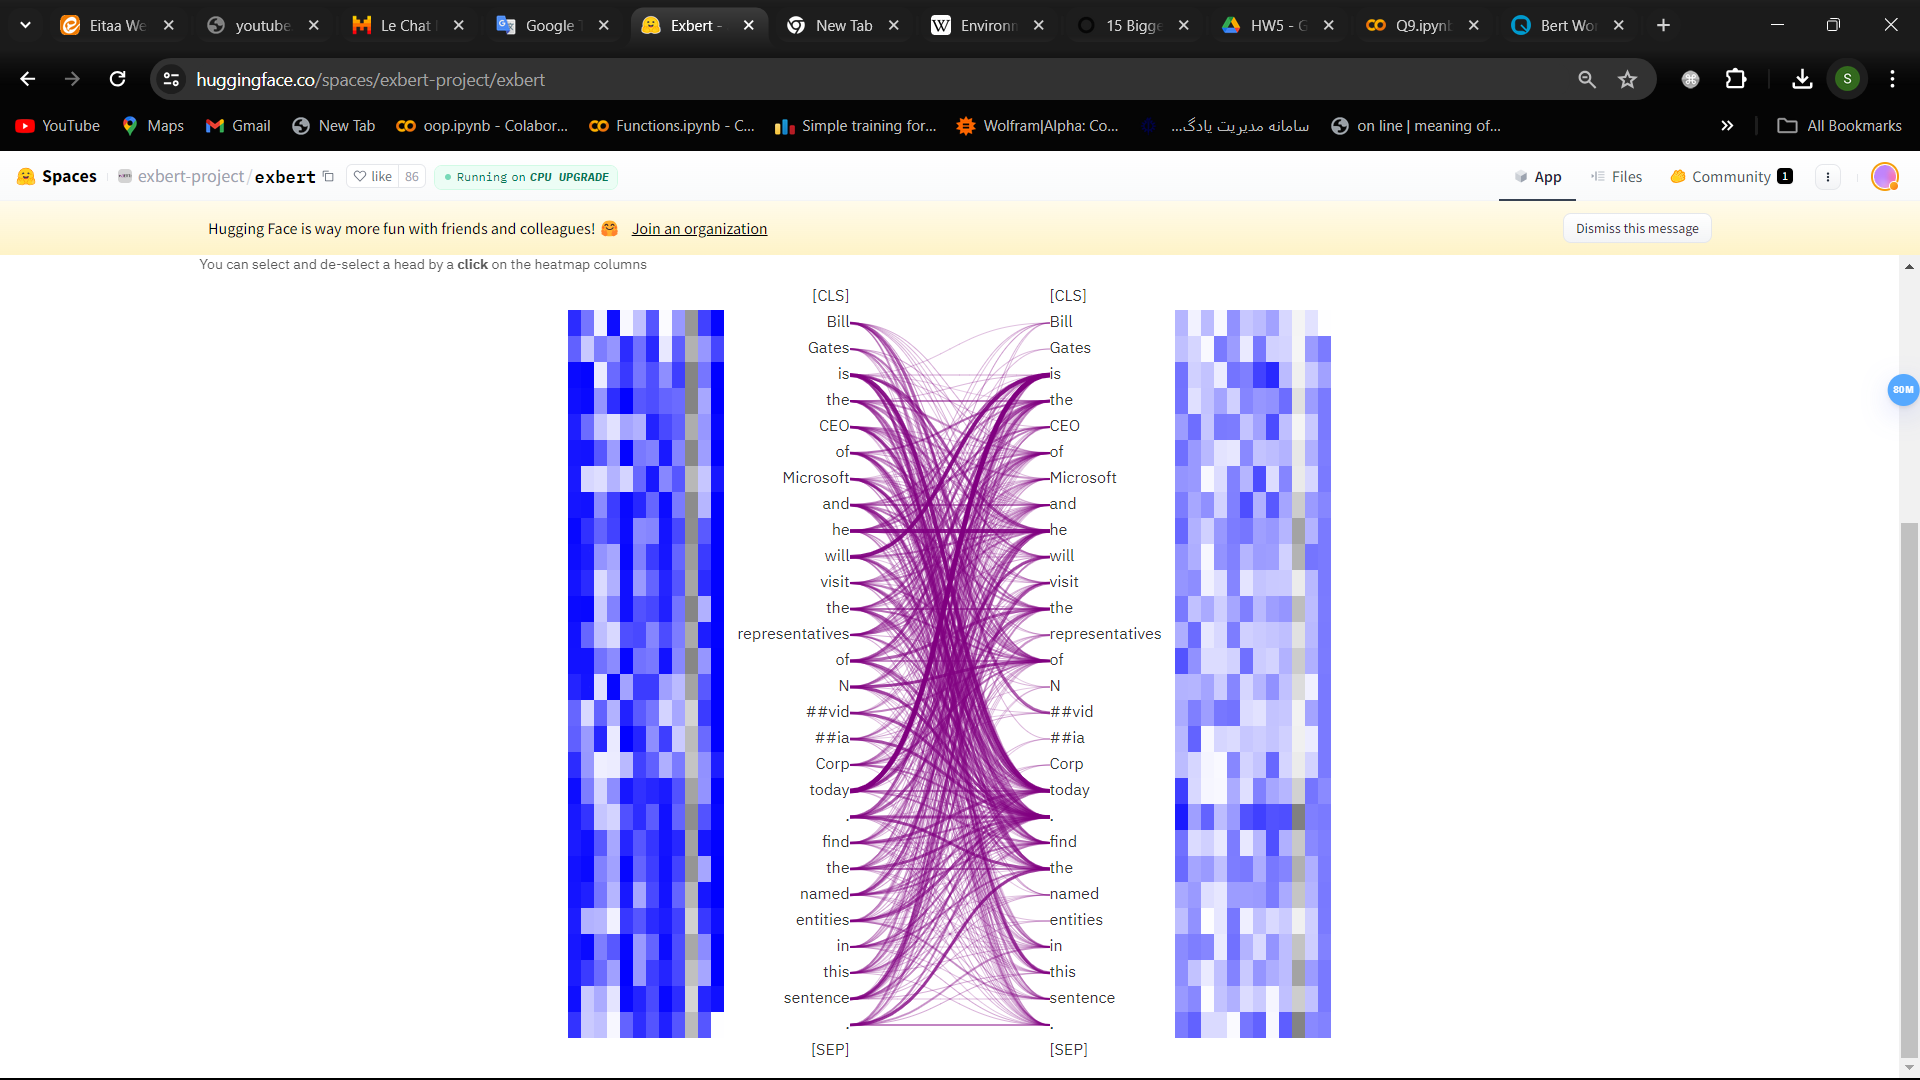
\includegraphics[width=0.5\textwidth]{188}\par\vspace{1cm}

\singlespacing
head شماره 4 

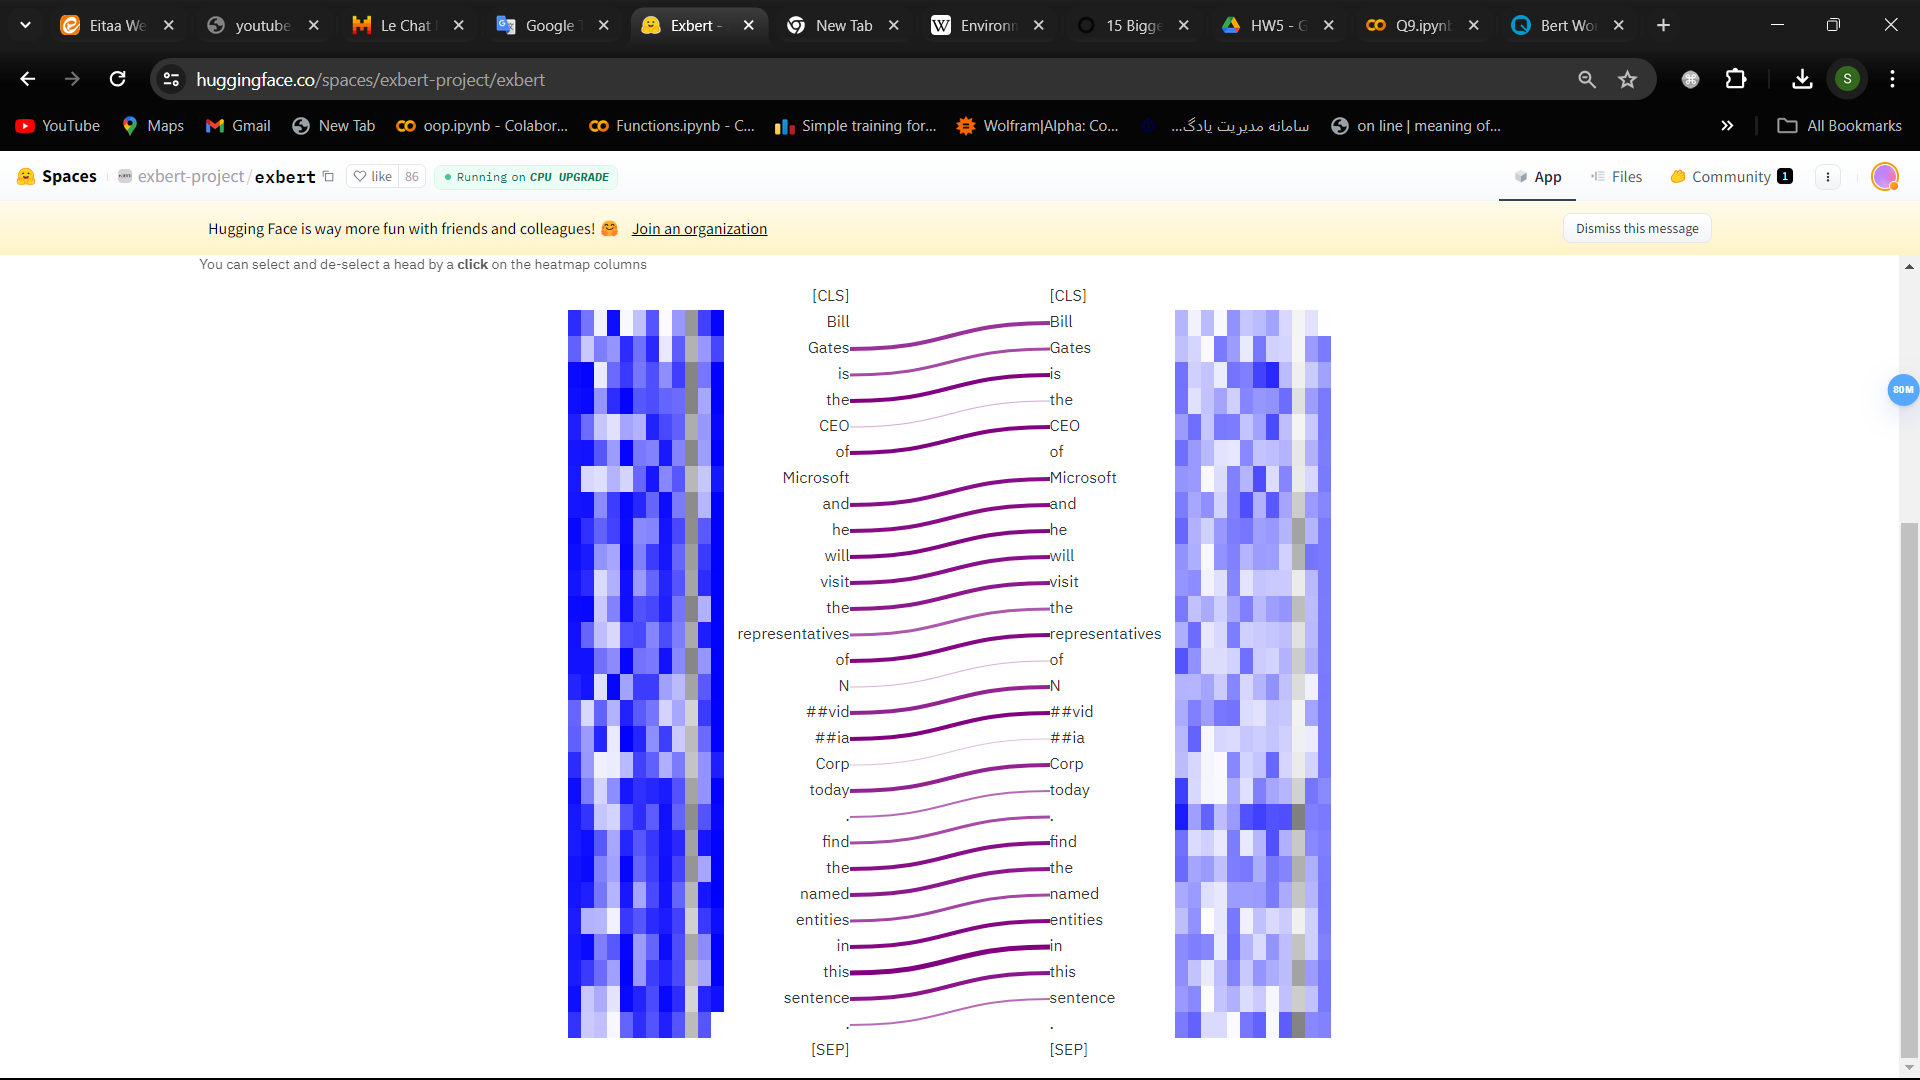
\includegraphics[width=0.5\textwidth]{189}\par\vspace{1cm}

head شماره 8 


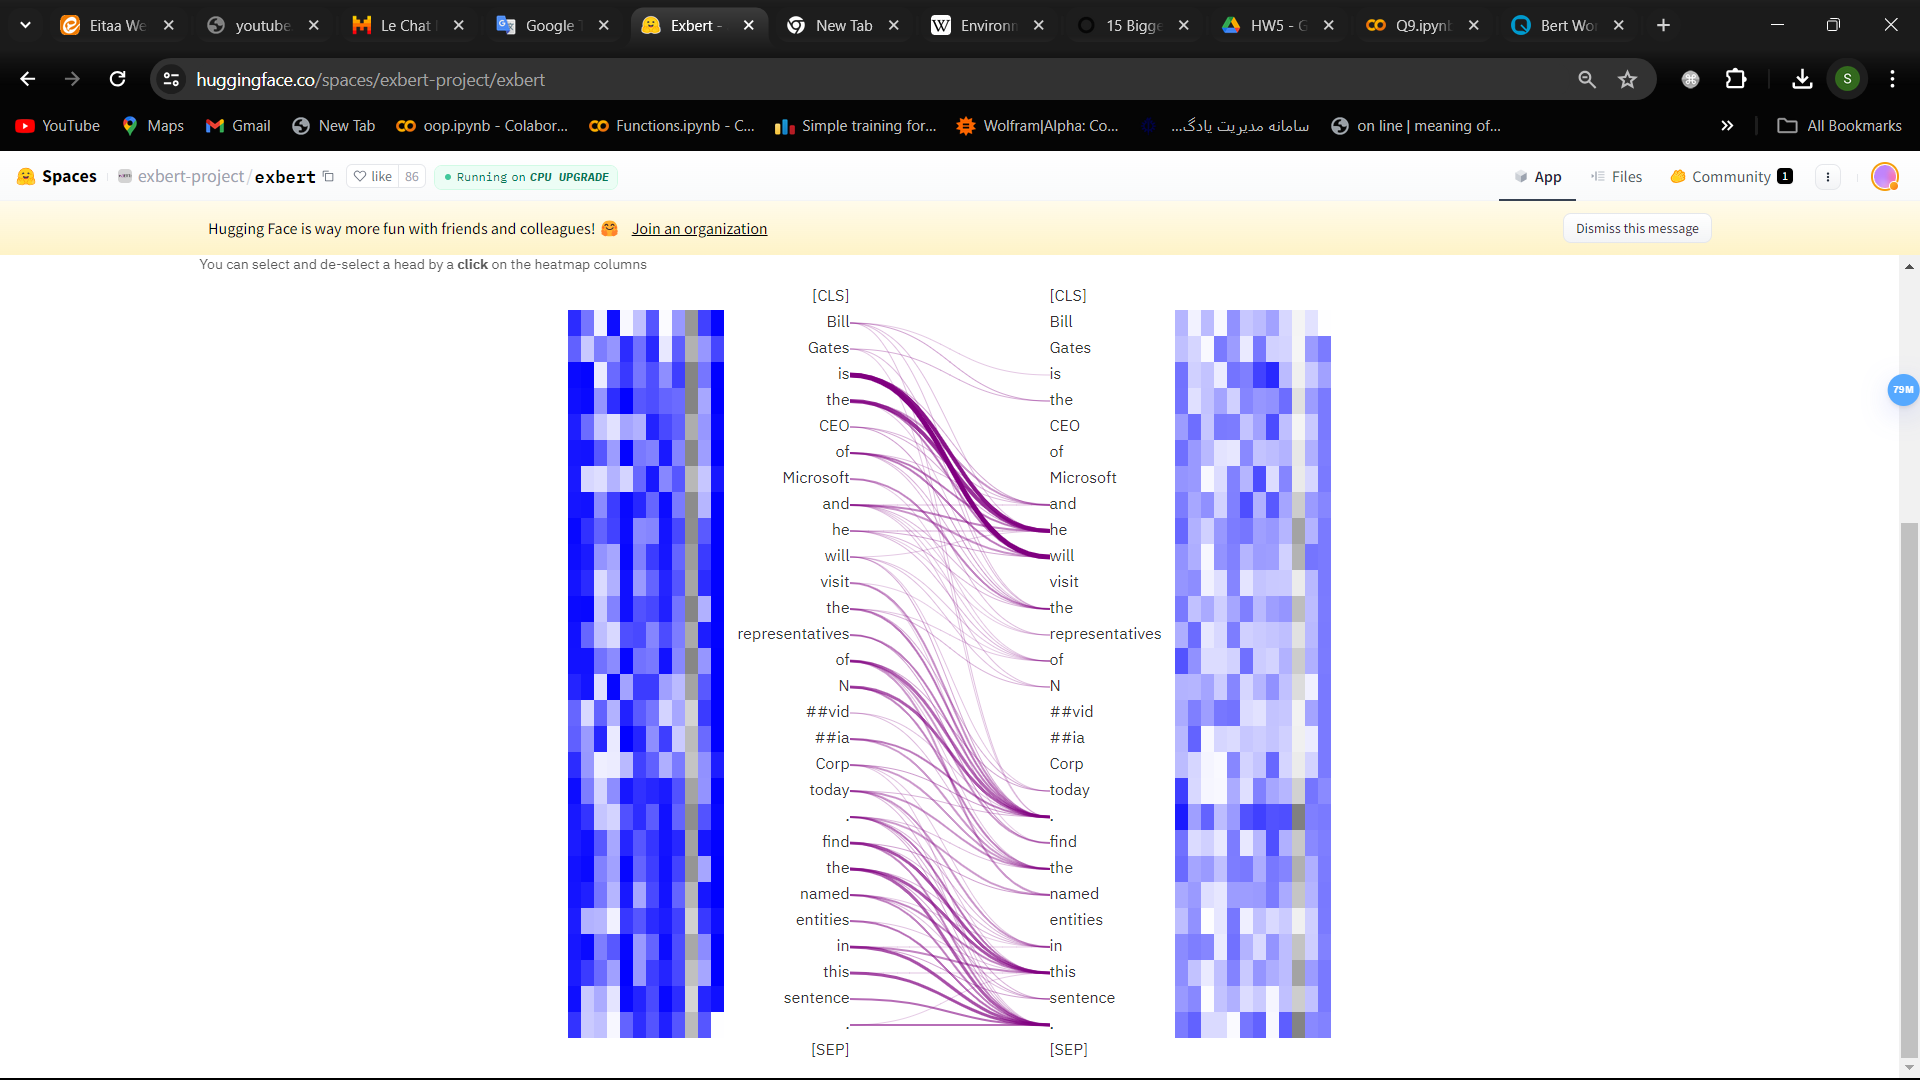
\includegraphics[width=0.5\textwidth]{190}\par\vspace{1cm}

head شماره 12 


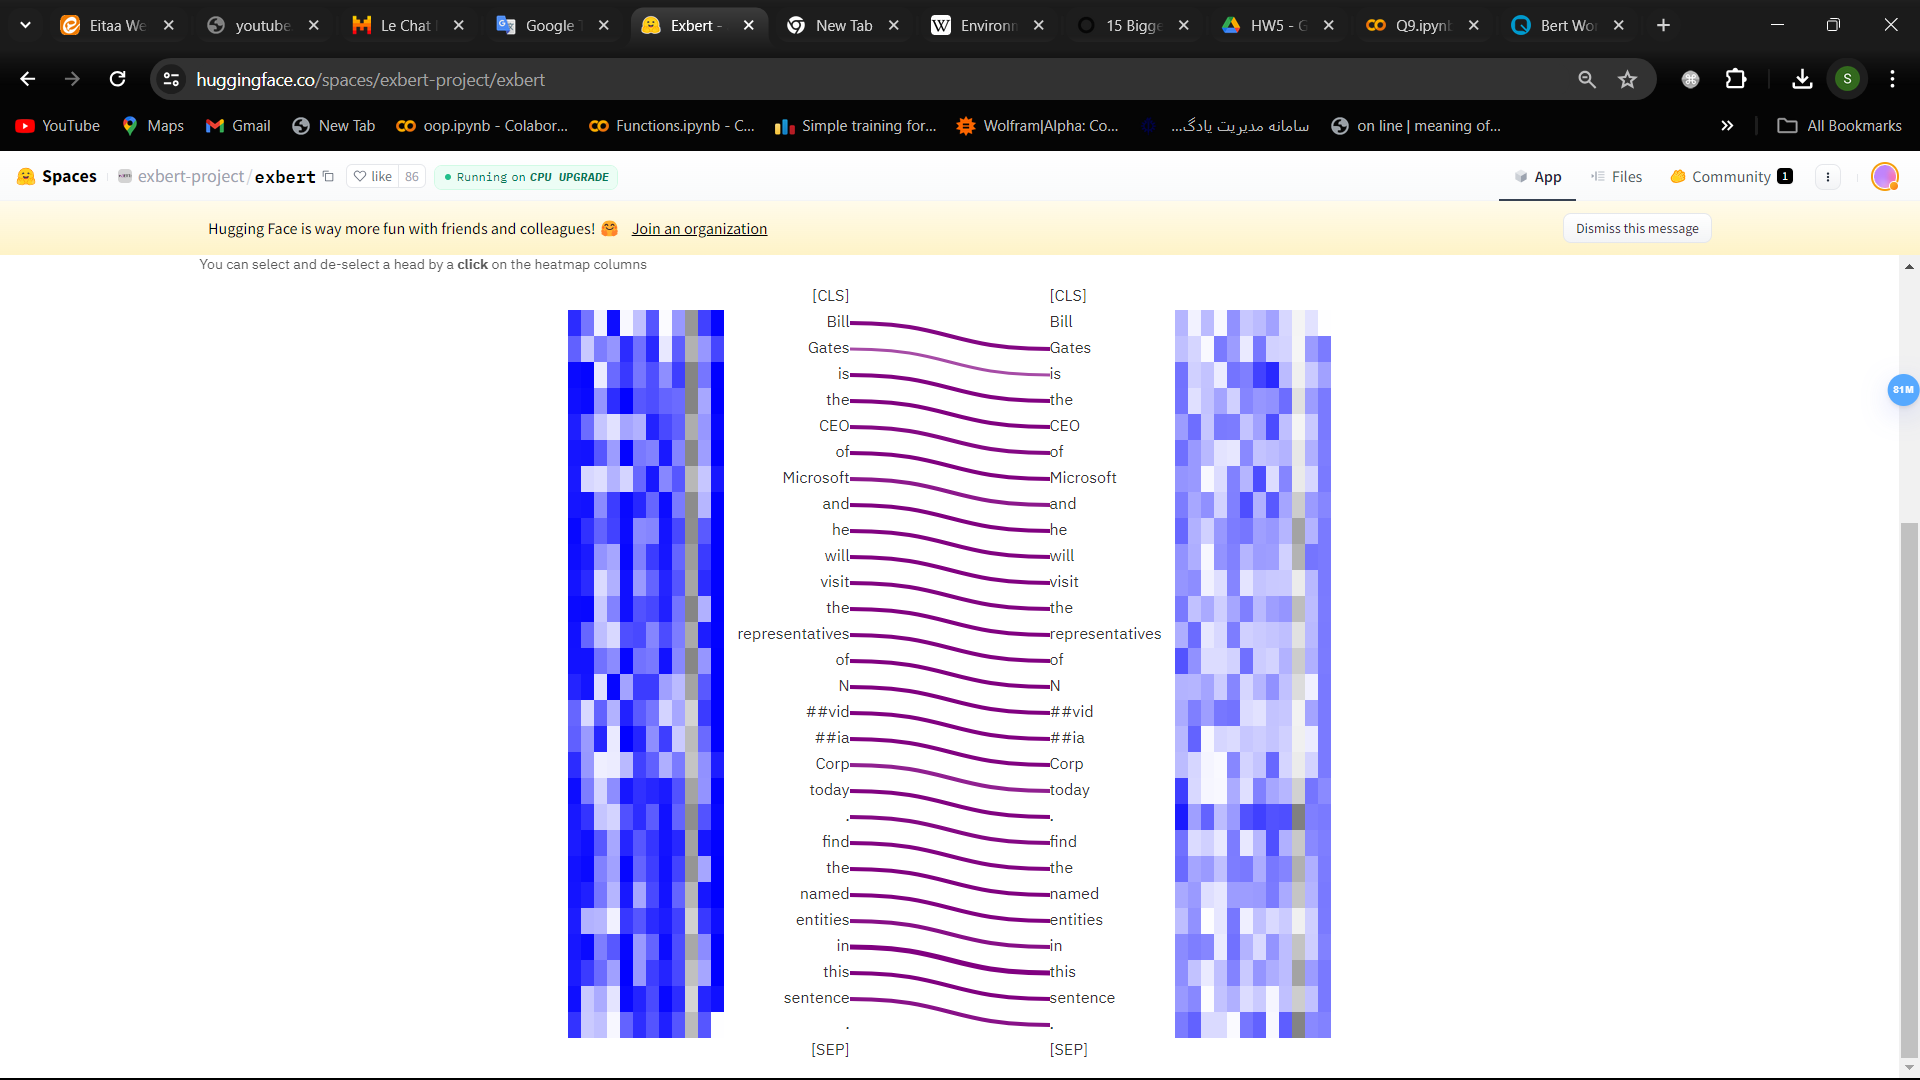
\includegraphics[width=0.5\textwidth]{191}\par\vspace{1cm}


\singlespacing


\setstretch{1.5}

\end{document}